%%
%% 研究報告用スイッチ
%% [techrep]
%%
%% 欧文表記無しのスイッチ(etitle,eabstractは任意)
%% [noauthor]
%%

%\documentclass[submit,techrep]{ipsj}
\documentclass[submit,techrep,noauthor]{ipsj}



% \usepackage[dvips]{graphicx}
\usepackage{latexsym}
\usepackage[dvipdfmx]{graphicx}
\usepackage{tabularx}
\usepackage{stfloats}
\usepackage{booktabs}

\newcommand{\todo}[1]{\colorbox{yellow}{{\bf TODO}:}{\color{red} {\textbf{[#1]}}}}
\newcommand{\ihara}[1]{\colorbox{green}{{\bf IHARA}:}{\color{blue} {\textbf{[#1]}}}}

\def\Underline{\setbox0\hbox\bgroup\let\\\endUnderline}
\def\endUnderline{\vphantom{y}\egroup\smash{\underline{\box0}}\\}
\def\|{\verb|}
%

%\setcounter{巻数}{59}%vol59=2018
%\setcounter{号数}{10}
%\setcounter{page}{1}


\begin{document}


\title{コードレビューにおける\\長期貢献者予測に向けた学習期間の検討}

\affiliate{IPSJ}{和歌山大学\\
Wakayama University}

\author{橋本 一輝}{Hashimoto Kazuki}{IPSJ}[s276189@wakayama-u.ac.jp]
\author{伊原 彰紀}{Ihara Akinori}{IPSJ}[ihara@wakayama-u.ac.jp]


\begin{abstract}
オープンソースソフトウェアプロジェクトでは,長期的に貢献する開発者(長期貢献者)が継続的な開発・保守において重要な役割を担っている.長期貢献者を早期に特定するためには,プロジェクト参加後の数ヶ月間の貢献の観察を要する.\todo{本研究では,それをなんとかするって言いたい}
本研究は,\todo{できれば参加後の数ヶ月を必要としない...みたいなこと言いたい}コードレビュー依頼を継続的に引き受ける長期貢献者を特定する手法を提案する.具体的には,逆強化学習を用いてレビュアーの貢献を学習し,継続的なコードレビュー依頼の受け入れ可否を決定する報酬関数を推定するモデルを構築する.ケーススタディとして,\todo{XXプロジェクトにおけるXXを対象とした結果,XXが明らかとなった.}
% オープンソースソフトウェアプロジェクトの継続的な開発・保守の実現には,長期的に貢献する開発者(長期貢献者)の確保が不可欠であるが,多くの開発者は数回の貢献後に活動が途絶えてしまうことが多い.従来研究では,長期貢献者を早期に特定する研究が進められており,プロジェクト参加後の数ヶ月の貢献に基づいて行われてきたが、コードレビュー作業への継続的な貢献を対象にした研究は進められていない.本研究では、コードレビュー依頼において,逆強化学習(IRL)を用いてレビュアーの貢献を学習し、継続的なタスク受け入れの判断を決定する報酬関数を推定する。
% 特に、レビュアーがタスクを受け入れる参加確率モデルの予測性能を検証するため、モデルの学習期間と貢献予測期間を動的に変更し、その予測精度と安定性を系統的に調査する。ケーススタディとしてコードレビュー履歴を対象に評価実験を行う.
% 本研究では,レビュアーの貢献が時間とともにどのように変化し、長期貢献者の予測に最適な学習期間を定量的に分析する。
\end{abstract}


%
\begin{jkeyword}
\todo{情報処理学会論文誌ジャーナル,\LaTeX,スタイルファイル,べからず集}
\end{jkeyword}
%
%\begin{eabstract}
%This document is a guide to prepare a draft for submitting to IPSJ
%Journal, and the final camera-ready manuscript of a paper to appear in
%IPSJ Journal, using {\LaTeX} and special style files.  Since this
%document itself is produced with the style files, it will help you to
%refer its source file which is distributed with the style files.
%\end{eabstract}
%
%\begin{ekeyword}
%IPSJ Journal, \LaTeX, style files, ``Dos and Dont's'' list
%\end{ekeyword}

\maketitle

%1
\section{はじめに}
オープンソースソフトウェア (OSS) は,地理的に分散した開発者によって実装,保守されているが,多くの開発者は,OSS開発組織から金銭的な利益を得ることなく,個人の知的好奇心や開発技術の学習などを動機として貢献している\todo{引用}.
%論文誌:OSS コミュニティにおけるオープンコラボレーションの理解
Raymondらは,OSS開発の成功例としてLinuxを対象に,このように不特定多数の開発者が自発的に参加する開発形態をバザール方式と名付けている\cite{bazaar}.この開発モデルは,多様な専門知識を有する開発者の参加を促進する一方で,開発者の流動性が極めて高い~\todo{引用}.
開発者の動機が多様なため,時間的制約や興味の変化によって数回の貢献後に活動を停止する開発者が多い\todo{one-time contributorを引用}.こうした開発者の離脱は,OSSプロジェクトの失敗の一要因になっている\cite{failed}

% オープンソースソフトウェア (OSS) は,世界中のボランティア開発者の貢献によって発展している.これらの貢献者は,営利的な目的ではなく,社会的・技術的など多様な動機に基づき,違いに知識を共有しながら開発を進めてきた.この開発モデルはRaymondが提唱した「伽藍とバザール」における「バザール」モデルに相当する\cite{bazaar}.この開発モデルでは,開発者の多様な参加を促進する一方で,開発者の流動性が極めて高いという課題を抱えている


OSSを長期的に運用,保守しているプロジェクトでは,長期的に貢献する長期的貢献者 (LTC) が重要な役割を担っている\todo{引用}.
% 書籍:K. Fogel, Producing open source software: How to run successful free software project, Sebastopol, CA, O'Reilly Media, 2005.
\todo{LTCの定義をここで書いておきたい}
LTCは,ソフトウェアの大部分を実装しているプロジェクトも存在する\todo{引用}.
%Evidence for the Pareto principle in Open Source Software Activity (Goeminne & Mens, 2011)
%Revisiting the applicability of the Pareto principle to core teams in open source software projects (Yamashita et al., 2015)
また,実装に限らず,新規参加した開発者のメンター\todo{引用},コードレビュー\todo{引用}などを行い,一部のLTCには,リポジトリの主要なブランチにコミットする権限が与えられ,プロジェクトの継続的な運用を支えている.このような経験が豊富なLTCは,流動性の高い組織構造を有するOSSプロジェクトに少数しか存在しないため,LTCに作業負担がかかることが少なくない\cite{related2}.LTCへの負担軽減のためにも,継続的に貢献する開発者の参加が喫緊の課題である\todo{引用}.


% プロジェクトを持続可能性を確保する上で重要なのが,プロジェクトに長期的に貢献する長期的貢献者(LTC)の存在である.LTCは単に新しいコードを作成するだけでなく,新規開発者の育成や,ソフトウェアコードレビューといったプロジェクトの中核的な役割を担う.コード作業やレビュープロセスには十分な知識を要するため,経験が豊富なLTCに作業が集中しやすい\cite{related2}.これらの問題を緩和するために,将来のLTC候補となる貢献者を特定し,候補者が離脱しないようサポートを行うことが重要である.



従来研究では,将来的にLTCとして長期間にわたってプロジェクトに参加する開発者を早期に特定する手法が提案されている\todo{引用}.\todo{XXらは}が開発したLTC候補者予測モデルは,プロジェクト参加後の1間月間の貢献を観察し\todo{XX}などのメトリクスを用いることで\todo{XX程度の精度で}LTCを特定することを実現している.しかし,LTCが担うタスクの1つであるコードレビュー作業への継続的な貢献に着目した研究は十分に進められていない.\todo{ではなくて,できれば参加後の数ヶ月を必要としない...みたいなこと言いたい}.本研究は,開発者が作業依頼の受け入れ,または依頼に反応しない記録を明確に取得可能なコードレビューを題材に,将来のコードレビュー依頼に対するレビュアーの貢献行動可否を,開発者の継続的な貢献と捉えたLTC候補者予測モデルを提案する.\todo{ここで,「受け入れは,開発者の興味,つまり継続的に貢献する意思がある,反応なしは継続的に貢献する意思がないことを意味する」みたいな,ことを書きたい.}具体的な予測モデルの構築には,\todo{(強化学習ではなく逆強化学習である理由)}のため,逆強化学習 (IRL: Inverse Reinforcement Learning) を用いる.本手法は,レビュアーがコードレビュー依頼を受け入れる際の判断指標\todo{判断指標?確率のこと?}(報酬関数)を推定し,継続的に貢献するレビュアーを予測するモデルを構築する.特に,モデルの学習方法,予測期間を変更することにより\todo{何から変更している?},予測精度と安定性\todo{安定性とは?}を調査することで,長期貢献者\todo{長期貢献者は予測しているのか?}の予測モデルの検討を行う.本手法を評価するために次の3つの Reseach Questions(RQs)に回答する.
\begin{itemize}
    \item RQ1:逆強化学習に基づく提案モデルは,コードレビューにおける長期貢献者\todo{長期貢献者なのか?}をどの程度予測できるか?
    \item RQ2:学習時のラベル\todo{ラベルとは?}の付け方・予測期間の長さに応じて,予測モデルの精度はどのように変化するか?
    \item RQ3:推定された報酬関数において、長期貢献者の継続的なタスク受け入れに寄与する特徴量(動機)\todo{RQ3のメッセージとして動機と捉えるのはいいけど,ここで動機と書くのは危険}は何か?
\end{itemize}


続く\ref{sec:related}章では,本研究の関連研究を紹介し,本研究の位置付けを明確にし,\ref{sec:ml}章では,本研究で用いる,逆強化学習とそれに関連する強化学習を紹介し,\ref{sec:model}章では,本研究の提案手法を述べ,\ref{sec:casestudy}章でケーススタディの結果を述べRQに回答する.\ref{sec:discussion}で本研究の結果を考察し,\ref{sec:conclusion}章で本研究をまとめる.




%%%%%%%%%%%%%%%%%%%%%%%%%%%%
%3
\section{関連研究}\label{sec:related}
%%%%%%%%%%%%%%%%%%%%%%%%%%%%

\subsection{OSSへ継続的に貢献する開発者の研究}

従来研究では,開発者が特定のプロジェクトで活動を継続する動機を調査している.Wuらによる定性的分析において,OSS開発者は利他的な動機(例: 貢献による名誉や実績)や人的資本の向上に関連する経済的動機(例:専門知識を有する開発者との協調)をもってOSSプロジェクトへの参加を継続していることを明らかにしている\todo{引用}.
%Wu CG, Gerlach Jh, Young CE (2007) An empirical analysis of open source software developers’ m0otivation and continuance intentions. Informatnion and Management 44(3):153–262
その他,多くの研究者がOSSプロジェクトにおける新規参加者の定着に影響を与える要因を調査してい\todo{引用4本}.
%Bird C, Gourley A, Devanbu P, Swaminathan A, Hsu G (2007) Open borders? immigration in open source projects. In: Proceedings of the 4th International Workshop on Mining Software Repositories (MSR’07), pp 6–13
%Jensen C, Scacchi W (2007) Role migration and advancement processes in OSSD projects: a comparative case study. In: Proceedings of the International Conference on Software Engineering (ICSE’07), pp 364–374
% Steinmacher I, Chaves AP, Gerosa MA (2013) Why do newcomers abandon open source software projects? In: Proceedings of the InrernationalWorkshop on Cooperative and Human Aspects of Software Engineering (CHASE’13), pp 25–32
%Zhou M, Mockus A (2012) What make long term contributors: willingness and opportunity in oss community. In: Proceedings of the 34th International Conference on Software Engineering (ICSE’12), pp 518–528

Birdらは,開発者がOSSプロジェクトに貢献する期間に影響を与える要因を理解するためのハザード率モデル(hazard-rate model)を提案している\todo{引用}.
%%Bird C, Gourley A, Devanbu P, Swaminathan A, Hsu G (2007) Open borders? immigration in open source projects. In: Proceedings of the 4th International Workshop on Mining Software Repositories (MSR’07), pp 6–13
ケーススタディとして,Apache,Python,PostgreSQLプロジェクトでは,特定のプロジェクトで約1年間活動した開発者をリポジトリの主要なブランチにコミットする権限を与えていることを示している.特に,ApacheおよびPythonプロジェクトでは,継続的にパッチを作成している開発者に権限を与えられていることを明らかにしている.このように,OSSプロジェクトは,LTC候補者に継続的な貢献を期待していることが確認できる.


\subsection{長期貢献者候補者の研究}

従来研究では,LTC候補者を予測する手法が提案されている.\todo{引用}
%Zhou M, Mockus A (2012) What make long term contributors: willingness and opportunity in oss community. In: Proceedings of the 34th International Conference on Software Engineering (ICSE’12), pp 518–528
Zhouらは,OSSプロジェクトに新規に参加した開発者の中からLTC候補者を特定するモデルを開発している\cite{related1}\todo{引用}.当該研究において,LTC候補者に分類される開発者は,技術的能力,意欲,および環境に依存することを明らかにしている.特に,LTC候補者を特定するためには,プロジェクト参加後の1間月間の貢献を観察し\todo{XX}などのメトリクスを用いることで\todo{XX程度の精度で}LTCを特定することを実現している.
%%Zhou M, Mockus A (2012) What make long term contributors: willingness and opportunity in oss community. In: Proceedings of the 34th International Conference on Software Engineering (ICSE’12), pp 518–528



ELuriらは,OSSプロジェクトに新規に貢献した開発者の特徴量,および貢献したリポジトリの特徴量に基づき,開発者が3年後に貢献しているか否かを予測するモデルを開発している\cite{related1}.提案モデルは,従来手法の予測精度に比べて非常に高く,AUCが0.913という結果を得ている.当該研究の比較対象とされたBaoらの研究も同様に,T年後 (T=1 ,2, 3) に開発者が貢献しているか否かを,プロジェクト参加直後1ヶ月間の貢献から予測モデルを構築している.これらの研究は,OSSの開発記録であるコミットやイシューへの対応など,プロジェクトでの全般的な活動を貢献とみなし,将来の単一時点での予測に留まっている.\todo{なぜ単一時点だとだめなの?橋本研究ではどうなの?}

% 彼らが比較対象としたBaoらの研究\cite{related2}も同様に,T年後(T=1 ,2, 3)に貢献者が存在しているかを,プロジェクト参加時点から1ヶ月間の活動から予測する研究であった.

% 者がプロジェクトに参加した時点で収集が可能な31個の特徴量(コントリビュータに関する特徴量18個,リポジトリの特徴量13個)を用いて,貢献者が3年後も活動があるかどうかを予測するモデルを作成した.予測には5つの機械学習モデルが使用され,その結果Ramdom Forestが最も優れた性能を示し,AUCは0.913であった.彼らが比較対象としたBaoらの研究\cite{related2}も同様に,T年後(T=1 ,2, 3)に貢献者が存在しているかを,プロジェクト参加時点から1ヶ月間の活動から予測する研究であった.
% これらの研究は,commitやissue対応といったプロジェクトでの全般的な活動を貢献とみなしている.また,予測においても将来の単一時点での予測に留まっている.

\subsection{開発者の離職予測に関する研究}

\todo{これって,前の節に混ぜてもいいのでは?}
従来研究は,開発者の離脱を予測する手法を提案している.Linらは,プロジェクトに参加直後の6ヶ月間の月次レポート\todo{月次レポートって何?}に基づき,1年後に離職しているか否かを予測するモデルを提案している\todo{引用}.評価実験の結果,ELuriらの研究と同様にRamdom Forestが最も優れた性能を示し,\todo{Random Forestのことは書かなくていいので消す予定ですが,RandomForestの精度がこんなに良いって書くなら,RandomForest使えばいいのに,って気になるw}.予測に寄与する特徴量には,月次レポートのタスク報告内容,労働時間の標準偏差,プロジェクト開発者での労働時間\todo{OSSじゃないの?どうやって計測したんやろ?}の標準偏差であった.この研究も同様に,月次レポートに基づく活動でありプロジェクトでの全般的な活動を貢献とみなしている.また,予測に関しても単一の時点である.

\ihara{ここまで修正済み}

\subsection{本研究の位置付け}
2.1及び2.2の従来研究は,コミットや月次レポートといったプロジェクトでの全般的な活動に基づき,単一時点での予測を行っており,LTCや開発者の定着性を予測する上で重要な知見を提供している.
ここで,本研究ではプロジェクトでの全般的な活動ではなく,コードレビュー作業というより専門的な活動に焦点を当て分析する.
また,予測においてもT年後という単一時点の予測から0-3ヶ月後,3-6ヶ月後,6-9ヶ月といった連続的な区間における貢献の有無を予測する.これにより,従来の研究では捉えることができなかった,貢献者が「いつ」活動し,「いつ」離脱するのかといった動的なパターンを捉えることを可能にすることを目的とする.具体的には.また,一度活動を休止した後に再び貢献するといったパターン(例:0-3ヶ月後は活動,3-6ヶ月後は休止,6-9ヶ月後に活動)を特定できる可能性がある.これにより,プロジェクトの管理者が,開発者が「いつ」離脱する可能性が高くなるか,あるいは復帰する可能性があるかを予測することができる.

%4
%%%%%%%%%%%%%%%%%%%%%%%%%%%%
\label{sec:ml}
\section{強化学習・逆強化学習}
%%%%%%%%%%%%%%%%%%%%%%%%%%%%

本研究では,逆強化学習を使用する.以下で強化学習と合わせて説明する.
\subsection{強化学習}
\begin{figure}[h]
    \centering
    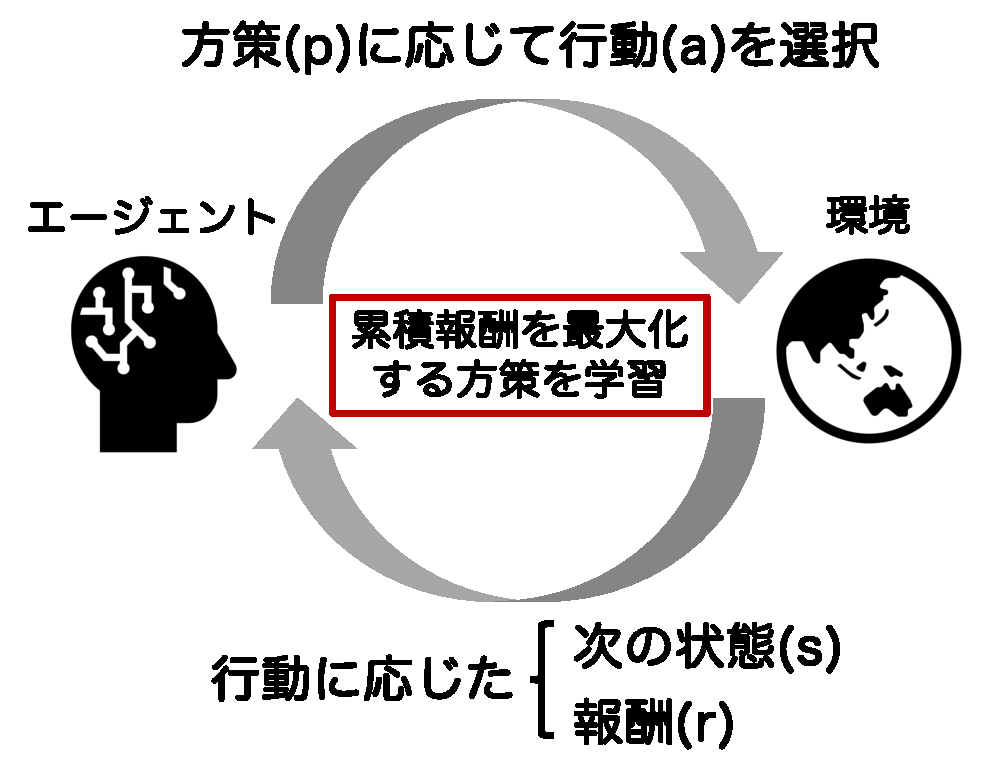
\includegraphics[width=1.0\linewidth]{./Hashimoto_fig/RL.pdf}
    \caption{強化学習のイメージ図}
    \label{fig:RL}
\end{figure}


強化学習(Reinforcement Learning, RL)は,エージェントと環境が相互作用を通じて,累積報酬を最大化するような行動の方策を学習する機械学習の一分野である.以下の基本的な構成要素から成る
\begin{itemize}
    \item エージェント:学習・意思決定を行う主体
    \item 環境:エージェントと相互作用する対象
    \item 状態:環境の現在状況(スナップショット)
    \item 行動:エージェントが取ることの選択肢
    \item 報酬:行動の良し悪しに応じて与えられるスカラー量
    \item 方策:エージェントの行動を決定する
\end{itemize}
強化学習において,報酬関数R(s,a)は最も重要な要素であり,報酬関数が,エージェントの達成するべきことを定義する.しかし,多くの実世界の問題では,複雑や要因が相互に作用しているため,事前に報酬関数を設計することは困難であり,報酬関数が不適切だと意図しない行動を学習してしまう.
\subsection{逆強化学習}
逆強化学習では,強化学習の事前に報酬関数を設計することが困難であるといった課題を解決するために,専門家の行動から,その行動を説明する報酬関数を逆算するアプローチをとる.既知の報酬関数から最適な方策を学習する強化学習に対して,逆強化学習は既知の専門家の軌跡から,その行動を説明する報酬関数を推定する.ここでの専門家の軌跡とは,状態と行動のペアを時系列に並べたものであり,専門家はある報酬関数(目的)を最大化するよう行動していると仮定し,その報酬関数を推定する.
\subsubsection{逆強化学習の強み}
従来の教師あり学習でのLTC予測では,単一時点でのスナップショットから予測を行うモデルを作成し,予測を行っていたため,過去の文脈の変化のパターンを捉えることが難しい.しかし,逆強化学習は,時系列の活動を軌跡として扱い,各状態と行動から報酬関数を推定するため,過去の行動パターンが将来の行動の予測に影響を与える.そのため従来では捉えることが難しかった,どのような行動パターンが継続につながるのかといった過去の文脈をより正確に捉えることができるため,本研究では逆強化学習を用いる


%%%%%%%%%%%%%%%%%%%%%%%%%%%%
%5
\section{長期貢献者予測モデル}
\label{sec:model}
%%%%%%%%%%%%%%%%%%%%%%%%%%%%
\subsection{データ収集}
\subsubsection{データソース}
本研究では,Gerrit REST APIを用いて,gerritからOpenStackプロジェクトのデータを取得した
\subsubsection{収集データ}
\begin{itemize}
    \item レビュー依頼(Change)
    \begin{itemize}
        \item 変更ID,プロジェクト名,作成日時,ステータス,コード変更量(追加/削除)
    \end{itemize}
\end{itemize}
\begin{itemize}
    \item レビュアー情報
    \begin{itemize}
        \item メールアドレス,名前,アサイン日時
    \end{itemize}
\end{itemize}
\begin{itemize}
    \item レビュー活動
    \begin{itemize}
        \item  レビューコメント内容,投票スコア,応答時刻
    \end{itemize}
\end{itemize}

\begin{itemize}
    \item 活動履歴
    \begin{itemize}
        \item  過去活動統計(レビュー回数,レビュー応答率,プロジェクト在籍日数)
    \end{itemize}
\end{itemize}
\begin{itemize}
    \item レビュアーとの相互用
    \begin{itemize}
        \item レビュアーと変更作成者間の過去の相互作用回数??
    \end{itemize}
\end{itemize}

\subsection{データ前処理}
収集したデータから自動化されたbotアカウント(CI/CD等)と判断されるものを除外した.全てのデータをrequest-time(レビュー依頼時刻)でソートし,時系列順に整列した.


\subsection{ラベル付}
\subsubsection{報酬関数}
\begin{figure}[h]
    \centering
    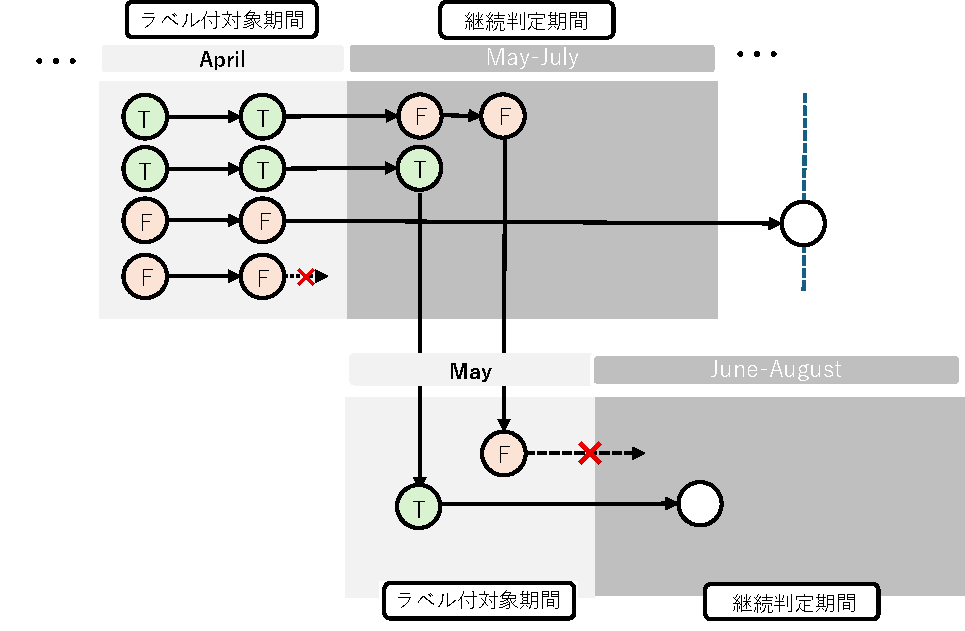
\includegraphics[width = 0.5\textwidth]{./Hashimoto_fig/label.pdf}
    \caption{図:指定期間が0-3mであった時のラベル付の例}
    \label{fig:label}
\end{figure}


本研究では,逆強化学習において,基準点からレビュアーが指定期間内に活動があるかどうかの二値変数でラベル付を行う.
\subsubsection{ラベルの基準点の設定}
レビュアーの活動ごとにラベルを付与すると,ラベルの数が膨大になり,学習時間の増加や,細かすぎるラベル付により類似した状態での学習が増加するため,過学習になる恐れがある.そのため,本研究では各月の末日を基準点とすることで,その月内の全活動に同一のラベルを付与する,これにより月単位での継続パターンを学習し,より一般化された予測モデルの構築を目指す.
\subsubsection{ラベル付の手順}
実際のラベル付は次の通りに行う.
\begin{enumerate}
    \item 活動日から活動月を特定する
    \begin{itemize}
        \item 例:2022-01-05 → 2022年1月
    \end{itemize}
    \item その月の最終日を基準点とする
    \begin{itemize}
        \item 例:2022-01-31
    \end{itemize}
    \item 基準点から指定期間の間で将来の活動があるか調べる(指定期間が0-3mの場合)
    \begin{itemize}
        \item 例:2022-01-31から2022-04-31に活動があるか(基準日から指定期間)
    \end{itemize}
    \item 活動があるかを判定
    \begin{itemize}
        \item 活動あり→True, 活動なし→False
    \end{itemize}
        \item その月の全活動に同じラベルを付与する(4)でTrueの場合
    \begin{itemize}
        \item 1月の全活動にTrueラベルを付与
    \end{itemize}
\end{enumerate}

\subsubsection{ラベルの学習時の役割}
このラベルは,逆強化学習の際に単なる過去の事実としてではなく,その時点での状態が,将来の継続とどう関連しているかを学習するための教師信号として機能する.具体的には,Trueのラベルからは,継続したレビュアーの活動から継続を促進する要因を学習し,Falseのラベルからは離脱したレビュアーのパターンから離脱のシグナルを学習することができる.

\subsection{特徴量抽出}
\subsubsection{状態・行動}
本研究では,9つの状態と,4つの行動特徴量を使用する.以下表でまとめる
\begin{table}[h]
    \centering
    \caption{状態特徴量(9次元)}
    \begin{tabular}{@{}ll@{}}
        \toprule
        \textbf{特徴量名} & \textbf{定義} \\
        \midrule
        \texttt{experience\_days} & 初回活動から現在までの日数 \\
        \texttt{total\_changes} & これまでの総コミット数 \\
        \texttt{total\_reviews} & これまでのレビュー数 \\
        \texttt{project\_count} & 参加したプロジェクト数 \\
        \texttt{recent\_activity\_frequency} & 30日間での活動数 \\
        \texttt{avg\_activity\_gap} & タイムスタンプ間の平均日数 \\
        \texttt{activity\_trend} & 月単位での活動量の差\\
        \texttt{collaboration\_score} & その開発者にレビューした数 \\ 
        \texttt{code\_quality\_score} & test/doc/refactor/fixの頻度 \\
        \bottomrule
    \end{tabular}
\end{table}

\begin{table}[h]
    \centering
    \caption{行動特徴量(4次元)}
        \begin{tabular}{@{}ll@{}}
        \toprule
        \textbf{特徴量名} & \textbf{定義} \\
        \midrule
        \texttt{intensity} & レビュータスクの変更行数 \\
        \texttt{message\_quality} & レビューリクエストのコメント内容 \\
        \texttt{collavoration} & パッチ作成者に対するレビュー依頼の応答率 \\
        \texttt{latency} & レビューリクエストから応答までの日数 \\
        \bottomrule
    \end{tabular}
\end{table}


\subsection{学習:損失関数と報酬関数の推定}
本研究のモデル学習は主に,目的関数である損失関数の設定と,逆強化学習(IRL)の原理に基づく報酬関数の最適化のプロセスから成る.
\subsubsection{損失関数:Focal Loss}
長期貢献者の予測というタスクにおいて,約8割の開発者が長期貢献者になる前に,離脱してしまうということが知られている[todo],そのため,正例と負例の間で学習データ数に不均衡が生じる.この不均衡問題を対処するために,本研究では,Focal Lossを使用する.
\subsubsection{Focal Lossの定義}
Focal Loss(FL)は,二値クロスエントロピー(BCE)において,クラスの不均衡が生じた際に,容易に分類できる学習ばかりが進み,難しいサンプルの学習にうまく焦点が当たらない問題を解決するために設計された.具体的んは,分類が容易である(正しく予測することができる)サンプルの損失の重みを小さくし,難しいサンプルに焦点が当たるように設計されている
\[\textbf{Binary Cross-Entropy (BCE)}\]
\[
L_{\mathrm{BCE}} = - \frac{1}{N} \sum_{i=1}^{N} \left[ y_i\log(p_i) + (1 - y_i)\log(1 - p_i)\right]
\]
ここで,
\[p_i = \sigma(z_i) = \frac{1}{1 + e^{-z_i}}\]はシグモイド関数であり,\(y_i \in \{0,1\}\) は正解ラベルを表す.

\todo{修正}
\[\textbf{Focal Loss (FL)}\]
\[
L_{\mathrm{FL}} = - \frac{1}{N} \sum_{i=1}^{N} \alpha (1 - p_i)^{\gamma} y_i \log(p_i) + (1 - \alpha) p_i^{\gamma} (1 - y_i) \log(1 - p_i)
\]

ここで,
\(\alpha \in [0,1]\) はクラス不均衡を補正する重みパラメータ,  
\(\gamma \ge 0\) は「難しいサンプルを強調する」焦点パラメータである.  
\(\gamma = 0\) のとき,Focal Loss は BCE に一致する.


\subsubsection{報酬関数}
\begin{figure*}[t]
    \centering
    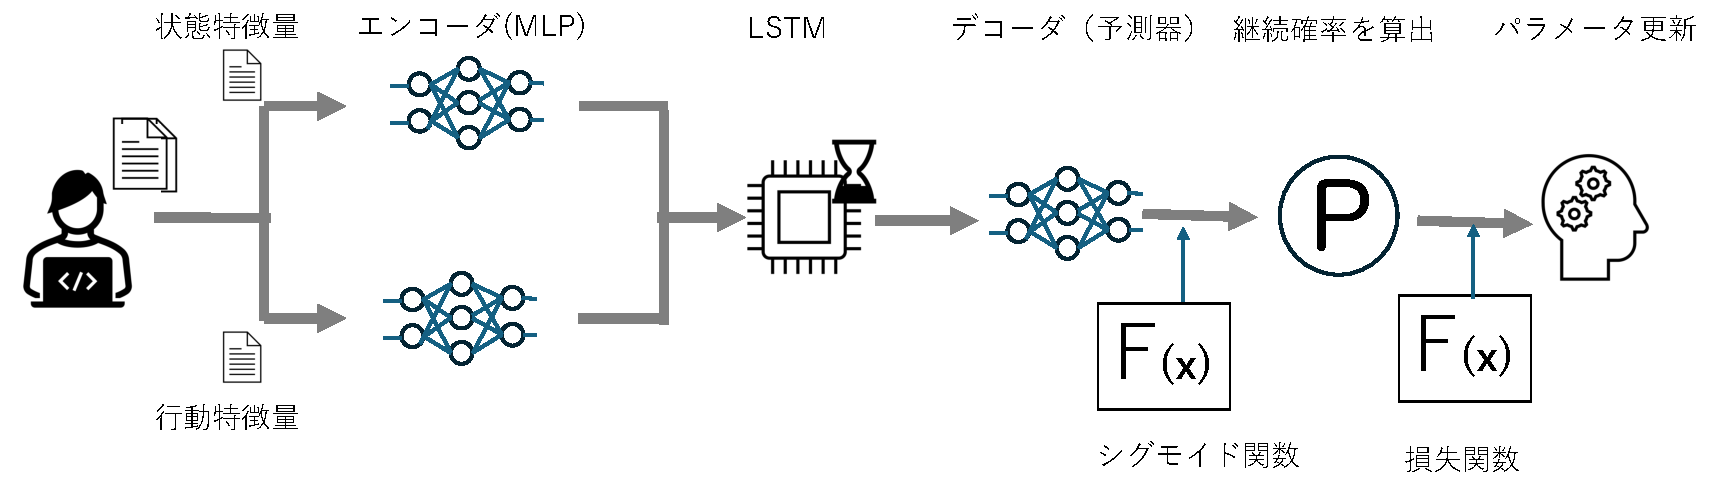
\includegraphics[width = 1.0\textwidth]{./Hashimoto_fig/prediction.pdf}
    \caption{図:学習から予測のフロー\todo{修正}}
    \label{fig:RL}
\end{figure*}

逆強化学習では専門家の行動を説明する報酬関数を学習する.具体的には,状態sで行動aを選択することの価値を表す報酬関数R(s,a;θ)を,ニューラルネットワーぅのパラメータθとして学習する.本研究での専門家は継続したレビュアーを指し,非専門家は離脱したレビュアーを指す.学習においては,専門家(継続者)の活動軌跡に対しては高い累積報酬を与え,非専門家(離脱者)の活動軌跡に対しては低い累積報酬を与えるように,報酬関数R(s,a;θ)を調整する.



\subsubsection{エンコーダと時系列処理}
学習に使用するネットワークは主に以下のものから構成される
\begin{itemize}
    \item エンコーダ
    \begin{itemize}
        \item レビュアーの各活動を表現している,状態(State),行動(Action)の2つの特徴量ベクトルをそれぞれ別の独立したエンコーダ(多層パーセプトロン:MLP)に入力する.これらのエンコーダは元のベクトルよりもより表現力のある高次元のベクトルに変換する役割を持つ.
    \end{itemize}
    \item LSTM
        \begin{itemize}
    \item 各時点tでエンコードされた状態・行動ベクトルを連結し,時系列プロセッサであるLSTM(Long Short-Term Memory)に入力する.LSTMは活動履歴を記憶し,時間的な依存関係を理解するため,単一の活動のみでなく,活動量が徐々に低下するといった動的なパターンを理解することができる.
    \end{itemize}
    \item デコーダ
    \begin{itemize}
        \item  LSTMによりレビュアーの全活動が処理された後に,MLP(予測器)で処理を行う.ここでは LSTMで処理されたレビュアーの全活動履歴を考慮した情報をデーコード(解釈)し,シグモイド関数により最終的な継続確率Pを算出する.
    \end{itemize}
\end{itemize}
\subsubsection{Focal Lossによる報酬関数の最適化}
4.5.4で算出される継続確率Pはシグモイド関数σを通して,軌跡の累積報酬todoに関連付いている.累積報酬が高いほど継続確率Pは高くなる.学習時には\todo{3章くらい}で定義した継続ラベルを活用し,この予測確率Pと継続ラベルの誤差を計算するために,\todo{前述}のFocal Lossを活用する.この誤差が最小となるように最適化アルゴリズム(Adam Optimizer)で反復してを行うことにより,継続者のパターンを高く評価し,離脱者のパターンを低く評価する報酬関数を作成する.




\subsection{予測・評価}
本研究では,学習時に予測時点以降の情報が用いられることを防ぐために,学習期間と予測期間を分離するだけでなく,特徴量計算に使用できるデータの最大時点(Max-date)を設けている.
具体的には,各時点においてはその時点以前のデータから特徴量を計算し,その月末の時点で継続ラベルを付与するが,Max-date以降のデータはラベル生成の際のみ使用する.これにより,モデルが将来の情報を事前に学習することを防ぐことができる.
ここで,最適化された報酬関数を用いて,特徴量に対する報酬を算出する.この報酬値にシグモイド関数を適応することで0~1の継続確率に変換することで予測を行う.


\subsubsection{評価指標}
 評価指標には,Pression,Recall,F1スコア,AUC-ROC(ROC 曲線下面積),AUC-PR(Precision-Recall 曲線下面積)の5つを用いる
 AUC-ROCでは,閾値に依存しない全体的な分類性能を評価し,継続者と離脱者を区別するモデルの基本的な能力を図る.さらに,本研究が用いるデータは,継続者(正例)と離脱者(負例)の差が顕著であり不均衡なクラスになっているため,不均衡なデータに対して予測性能をより適切に評価できることが知られているAUC-PRを使用する.本研究ではこのAUC-ROCの値を重視する.

\subsubsection{クロス評価}
従来研究では,将来の任意の時点以降の活動の有無を予測していたが,本研究では,将来の任意の区間での活動の有無の予測を行い,この区間をスライドさせて予測を行う.また学習時のラベル付に置いても,同様に区間をスライドさせて評価行う.
具体的には,学習時のラベル付の区間をスライドさせた4パターン(0-3m, 3-6m, 6-9m, 9-12m)のモデルで,予測区間をスライドさせた4パターン(0-3m, 3-6m, 6-9m, 9-12m)の16パターンで評価を行う.


%%%%%%%%%%%%%%%%%%%%%%%%%%%%
\section{ケーススタディ}
\label{sec:casestudy}
%%%%%%%%%%%%%%%%%%%%%%%%%%%%

\subsection{データセット}
\subsubsection{対象プロジェクト}
本研究では,仮想マシンインスタンスのプロビジョニングとライフサイクル管理を行う,OpenStackの中核的なコンピュートサービスOpenStack/Novaを対象とした.
\subsubsection{実験設計}
\begin{table}[h]
    \centering
    \caption{データセットの概要}
    \begin{tabularx}{\columnwidth}{XX}
        \hline
        項目 & 値 \\
        \hline
        対象期間 & 2021-01-01 ~ 2024-01-01 \\
        学習期間 & 2021-01-01 ~ 2023-01-01 \\
        予測期間 & 2023-01-01 ~ 2024-01-01 \\
        \hline
        総レビュー依頼数 & 約10,908件 \\
        訓練時レビュアー数 & 241人 \\
        予測時レビュアー数 & 167人 \\
        \hline
    \end{tabularx}
    \label{table:dataset}
\end{table}




\subsection{RQ1:逆強化学習に基づく提案モデルは,コードレビューにおける長期貢献者をどの程度予測できるか?}
\begin{table}[h]
    \centering
    \caption{0-0mモデルで0-0m後の貢献を予測した結果}
    \begin{tabularx}{\columnwidth}{XXXXX}
        \hline
       Precision & Recall & F1 & AUC-ROC & AUC-PR \\
       \hline
       0.694  & 0.806 & 0.746 & 0.746 & 0.\\
       \hline
    \end{tabularx}
\end{table}
表の結果が示す通り,AUC-ROCが0.787となりランダム予測(0.500)を大きく上回り,提案モデルがレビュアーの継続者と離脱者を効果的に区別できることを示している.本研究で重視しているAUC-PRは0.697となり,少数クラス(継続者)に対しても高い予測精度を発揮していることを示している.

\subsection{RQ2:学習時のラベルの付け方・予測期間の長さに応じて,予測モデルの精度はどのように変化するか?}
\begin{figure*}[t]
    \centering
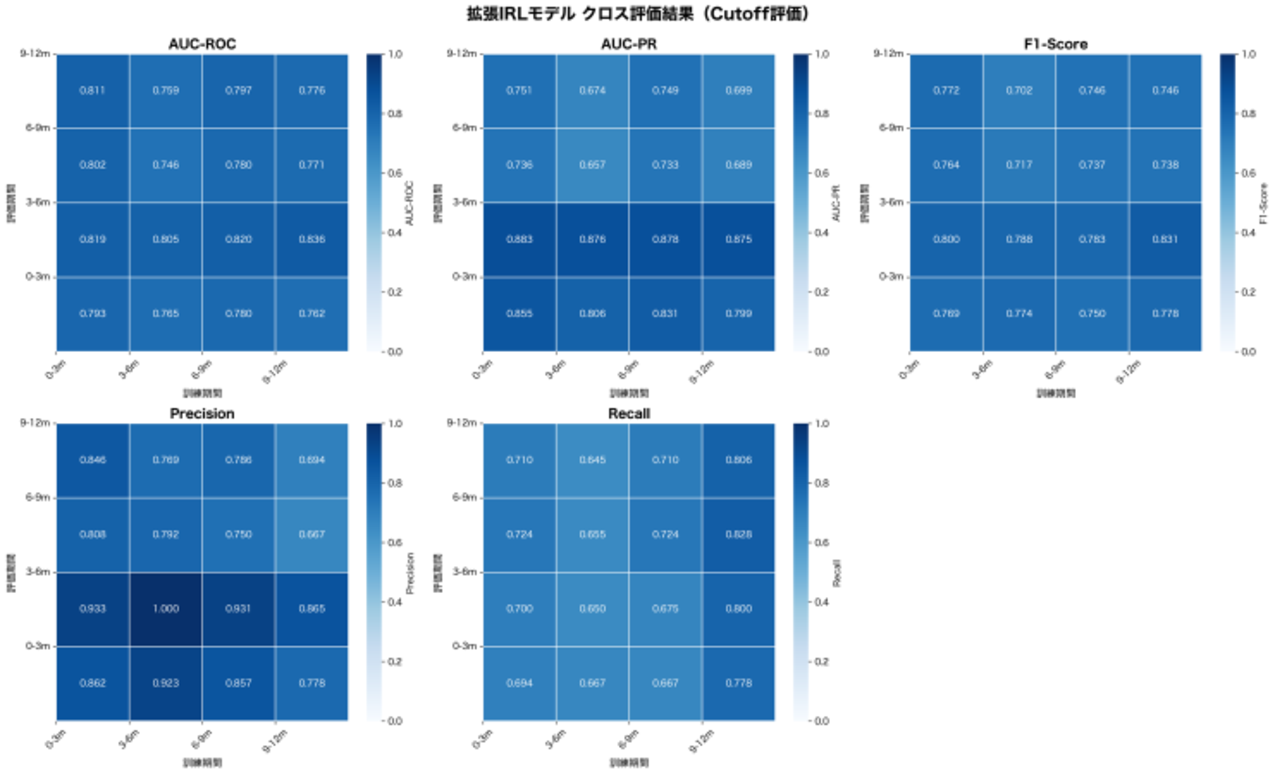
\includegraphics[width=1.0\textwidth]{./Hashimoto_fig/heatmap.pdf}
    \caption{各モデルのクロス評価(左:AUC,右:Recall)}
    \label{fig:Approach}
\end{figure*}
図\todo{番号}のヒートマップの縦軸は予測する区間をスライドさせたものであり,縦軸は学習時に付与するラベルの指定期間をスライドさせ評価指標の5つでヒートマップを作成した結果である.どの予測モデルにおいてもAUC-PRが
学習時のラベル付の期間と予測期間が一致する際に予測精度が最も高くなることが予想されていたが,結果として,全てのモデルにおいて,予測期間3-6mでAUC-PRが最大になった.他の予測期間においても,全てのモデルで同様の結果が見られ,AUC-PRが高いものから順に並べると3-6m, 0-3m, 9-12m, 6-9mの順になった.


\subsection{RQ3:推定された報酬関数において、長期貢献者の継続的なタスク受け入れに寄与する特徴量(動機)は何か?}
図5,6は報酬関数における,状態特徴量と行動特徴量の各特徴量の重要度をそれぞれ分析したものである.図5からは,レビュアーの継続を予測する状態特徴量として,最近の活動頻度が最も強い正の影響を与えていることが明らかになった.次で,平均活動間隔が開発者の予測に強い負の影響を与えることがわかった.
図6からは,レビュアーの継続を予測する行動特徴量として,レスポンス時間,協力度,品質,強度の全てにおいて負の影響を与えることが明らかになった.中でも強度が最もレビュアーの継続を予測する上で負の影響があることが明らかになった.

\begin{figure}[h]
    \centering
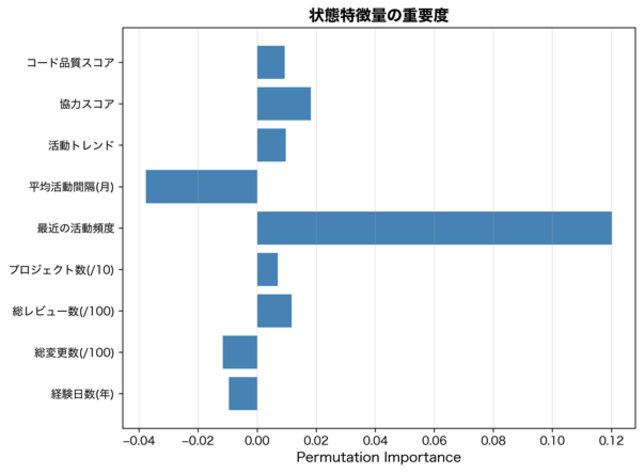
\includegraphics[width=0.5\textwidth]{./Hashimoto_fig/state.pdf}
    \caption{状態特徴量の重要度}
    \label{fig:State}
\end{figure}

\begin{figure}[h]
    \centering
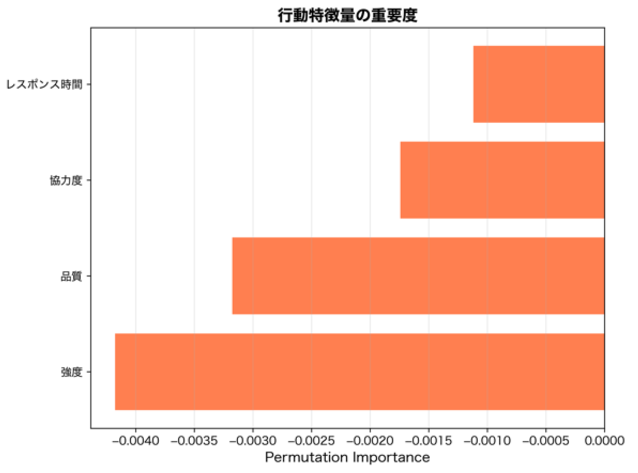
\includegraphics[width=0.5\textwidth]{./Hashimoto_fig/action.pdf}
    \caption{行動特徴量の重要度}
    \label{fig:Action}
\end{figure}


%%%%%%%%%%%%%%%%%%%%%%%%%%%%
\section{考察}
\label{sec:discussion}
%%%%%%%%%%%%%%%%%%%%%%%%%%%%
\subsection{\todo{RQの考察?}}
RQ2において全てのモデルで予測期間が3-6mでAUC-PRが最大であった原因として,予測期間が0-3mの場合は,レビュアーの離脱が多いため,ノイズが多く予測が難しく,予測期間6-9m, 9-12mにおいては,学習に用いたデータから予測する時点までの期間が遠くなるため予測が困難になるからであると考えられる.RQ3において,総レビュー数,レビュー負荷,レスポンス時間が負の重要度をもつため,レビュアーに負荷が集中し,レビューやレスポンスが遅延することによりレビュアーが離脱することが示唆された.

\subsection{妥当性の脅威}
本研究では,OpenStack/Novaという単一プロジェクトを対象としている.OpenStack/Novaは独自の開発形態やレビュープロセスを持っており,本研究で得られた結果が,他のドメインや開発プロセスを持つプロジェクト(例:GitHubを使用しているプロジェクなど)においては,今回の結果とは異なる新たな知見が得られる可能性がある.
また,0-3m,3-6m...3ヶ月単位で指定した将来の区間における活動の有無という二値分類を行なったが,この3ヶ月という区切り方が適切でない可能性がある.また,継続の予測に用いた状態・行動特徴量がレビュアーの継続要因の全てを満たしているわけではない.

%%%%%%%%%%%%%%%%%%%%%%%%%%%%
\section{おわりに}
\label{sec:conclusion}
%%%%%%%%%%%%%%%%%%%%%%%%%%%%

\todo{}

\begin{acknowledgment}
hogehoge
\end{acknowledgment}


\bibliographystyle{ipsjunsrt}
\bibliography{references}


\end{document}

